\documentclass[A5paper, 11pt]{article}
\usepackage[utf8]{inputenc}
\usepackage[spanish]{babel}
\usepackage{xcolor}
\usepackage[lmargin=3cm, rmargin=2.5cm, tmargin=5cm, bmargin=5cm]{geometry}
\usepackage[rightcap]{sidecap}
\usepackage{fancyhdr}
\usepackage{graphicx}
\usepackage{caption}

\author{Emiliano Gutiérrez Luengas}
\date{September 2022}

\begin{document}

\pagestyle{fancy}

\pagecolor{gray}

\hspace{5cm}{\huge\textbf{Rese\~na de serie:}}

\hspace{3cm}{\Large\emph{Erased}, una maravilla que resulta ser obra}
\lhead{Emiliano Guti\'errez Luengas}
\rfoot{\thepage}
\section{\emph{Serie}}
  \subsection{\textit{Rese\~na General}}
\emph{Erased}, o conocido en espa\~nol como \emph{Desaparecido}, es una serie anime corta de doce cap\'itulos. La trama principal gira en torno al protagonista, Satoru fujinuma, el cual posee un poder especial: tiene la capacidad de regresar en el tiempo para evitar tragedias. Por giros del destino, termina regresando 18 a\~nos al pasado, debido a que su madre es asesinada por un criminal ped\'ofilo que estuvo activo en su primaria. Con el fin de evitar ese cruel final, Satoru se embarca en una aventura para proteger a la que en su momento fue su compan\~nera de la infancia, Kayo Hinazuki, de su mortal desenlace a manos del violador.

{\tiny{\hspace{-3.5cm}- 'Creer' es una

\hspace{-3.5cm} palabra extraña,

\hspace{-3.5cm} porque si de

\hspace{-3.5cm} verdad crees en

\hspace{-3.5cm }algo o en alguien,

\hspace{-3.5cm} no necesitas decirlo

\hspace{-3.5cm} No decimos que

\hspace{-3.5cm} 'creemos' en el

\hspace{-3.5cm} aire.


\hspace{-3.5cm} - Así que creemos

\hspace{-3.5cm} porque desconfiamos,

\hspace{-3.5cm}  ¿no?

\hspace{-3.5cm} - No quiero decir

\hspace{-3.5cm} que creer en algo

\hspace{-3.5cm} sea una mentira.

\hspace{-3.5cm} Solo digo que

\hspace{-3.5cm} decimos que 'creemos'

\hspace{-3.5cm} cuando en realidad

\hspace{-3.5cm} queremos creer.}}

La trama, aunque no parece excesivamente compleja, es tratada de manera ilustre por el estudio de animaci\'on, adem\'as de seguir de manera casi fiel a la obra original. El desarrollo de personajes es sublime. Primero, la obra opta por poner al protagonista a una posici\'on de vulnerabilidad sumamente grande, enfrent\'andose a la persona que mat\'o a su madre y ocasion\'o que lo persiga la polic\'ia. Mas, cuenta con mucho menos poder que en el presente, y donde cada error cometido se paga con creces.

El final de la obra es su momento m\'as d\'ebil, pero sigue siendo impactante para el espectador, en lo que a c\'umulo de emociones se refiere. Es una obra recomendada profundamente, la cual f\'acilmente recibe una calificaci\'on de 4.5 de 5.

  \subsection{\textit{Elenco}}
\subsubsection{Autor y Estudio de animaci\'on}
\begin{enumerate}
    \item Autor: Kei Sanbe
    \item Estudio de animaci\'on: A-1 Pictures
    \item Cadena televisiva: Fuji TV (NoitaminA)
\end{enumerate}

 \subsubsection{Actores de doblaje paticipantes}
 \begin{enumerate}
      \item Voz de Satoru Fujinuma: Shinnosuke Mitsushima
      \item Voz de Satoru Fujinuma (chico): Tao Tsuchiya
      \item Voz de Airi Katagiri: Chinatsu Akasaki
      \item Voz de Kayo Hinazuki: Aoi Yūki
      \item Voz de Sachiko Funijuma: Minami Takayama
      \item Voz de Kenya Kobayashi: Jin Shirasu
      \item Voz de Osamu: Ayaka Nanase
      \item Voz de kazu: Yukitoshi Kikuchi
      \item Voz de Hiromi Sugita: Akari Kito
      \item Voz de aya Nakanishi: Sayaka Kaneko
      \item Voz de Jun Shiratori: Takahiro Mizushima
      \item Voz de Gaku Yashiro Mitsuru Miyamoto

\end{enumerate}

  \subsection{\textit{Personajes}}
\begin{itemize}
    \item \fcolorbox{gray}{cyan}{Satoru Fujinuma}
    \item \fcolorbox{gray}{orange}{Airi Katagiri}
    \item \fcolorbox{gray}{blue}{\textcolor{white}{Kayo Hinazuki}}
    \item Sachiko Fujinuma
    \item Kenya Kobayashi
    \item Osamu 
    \item Kazu 
    \item Hiromi Sugita
    \item Aya Nakanishi
    \item Jun Shiratori
    \item \fcolorbox{gray}{black}{\textcolor{white}{Gaku Yashiro}}
\end{itemize}

\newpage
  \subsection{\textit{Im\'agenes de la serie}}
  
  \begin{SCfigure}[h]
     \begin{flushright}
      \caption*{Erased: portada promocional}\\
      
      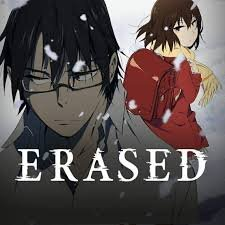
\includegraphics[scale=0.008, angle=15]{images (1).jpg}
    \end{flushright}
  \end{SCfigure}



\section{\emph{Razones de mi elecci\'on}}
La raz\'on principal de mi elecci\'on fue el recuerdo de la emoci\'on que me ocasion\'o cuando la vi ya hace muchos a\~nos. \textcolor{red}{El desarrollo de los eventos, poco predecibles, y algo fuera de lo ordinario para aquel chico de 12, acostumbrado a series del momento, le permitieron a \emph{Erased} ganarse un lugar en mi memoria.} La recuerdo con a\~noro y, pensando de que serie hablar, fue la que se me vino a la mente.

De igual manera, \textcolor{cyan}{la obra no se limita en expandir donde no debe y va directo al punto. es clara con su inenci\'on y, por lo tanto, mantiene conruencia a trav\'es de cada cap\'itulo. No siente uno, como espectador, que se desvie la trama o que los personajes actuen poco naturales. En pocas palabras, se logra formar un pacto de verosimilitud con el mundo de la obra.}

Finalmente, \textcolor{orange}{la dicotom\'ia entre el mundo de 18 a\~nos en el pasado, alegre y fr\'ivolo, chocan bruscamente con la realidad de la problem\'atica, haciendo cada vez m\'as presente el peligro en el que se encuentra el protagonista. Este contraste acentua cada detalle y lo amplifica, teniendo como resultado un impacto emocional superior sobre el espectador.}

\begin{figure}[h]
        \centering
        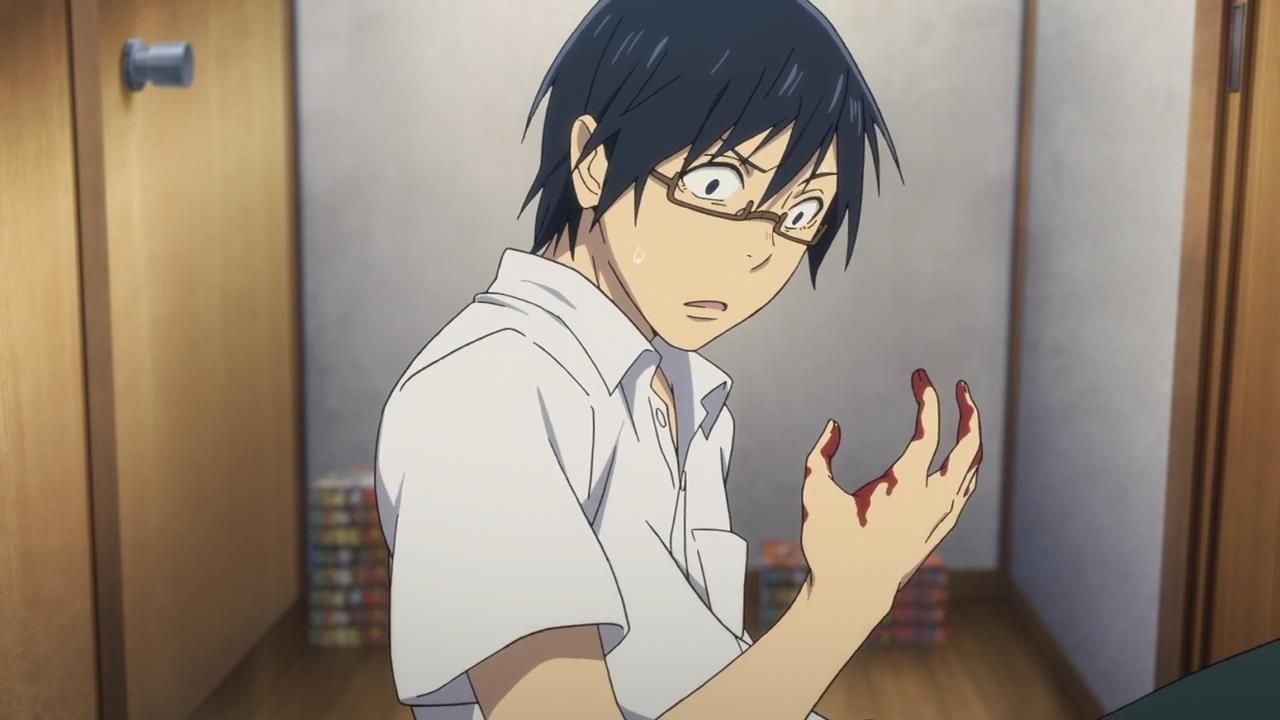
\includegraphics[scale=0.2, angle=-18]{Satoru funijuma.jpg}
        \caption*{Satoru Funijuma: Protagonista de la obra}
    \end{figure}
\begin{figure}[h]
        \centering
        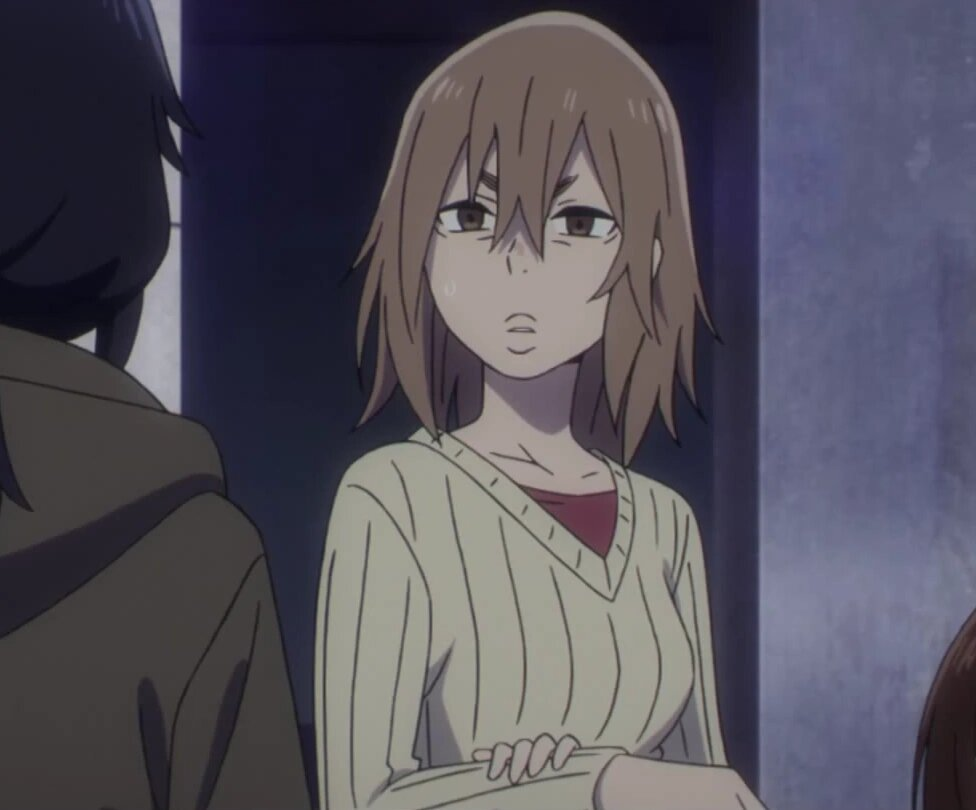
\includegraphics[scale=0.2, angle=8]{Hündin (1).jpg}
        \caption*{Madre de Kayo Hinazuki: Abusadora que no merece ni ser llamada desperdicio.}
    \end{figure}
        



\end{document}
